\documentclass[12pt]{article}
\usepackage{hyperref}
\usepackage{amsmath, amssymb, amsfonts}
\usepackage[margin=1.2cm]{geometry}
\usepackage{xcolor}
\usepackage{graphicx}
\usepackage{enumitem, inconsolata}
\usepackage{tikz}
\usepackage{circuitikz}[scale=1.2]
\usetikzlibrary{patterns}
\parindent 0px
\newcommand{\W}{\(\Omega\)}
\newcommand{\w}{\(\omega\)}
\newcommand{\lb}{\\$\left|\rightarrow\right.$}
\newcommand{\enter}{\\\textcolor{white}{1}}
\newcommand{\sub}[1]{\textsubscript{#1}}
\newcommand{\super}[1]{\textsuperscript{#1}}
\ExplSyntaxOn
\NewDocumentCommand{\bo}{m}
 {
   \bold_commas:n { #1 }
 }

\cs_new:Npn \bold_commas:n #1
 {
   \seq_set_split:Nnn \l_tmpa_seq { , } { #1 }
   \seq_map_indexed_function:NN \l_tmpa_seq \__bold_commas_aux:nn
 }

\cs_new:Npn \__bold_commas_aux:nn #1 #2
 {
   \textbf{#2}
   \int_compare:nNnTF { #1 } < { \seq_count:N \l_tmpa_seq }
     { , }
     { }
 }

\ExplSyntaxOff

\title{Embedded System}
\author{by PUL079BEI008\\by PUL079BEI014}
\date{\today}

\begin{document}
\maketitle
\vspace{10.5cm}
\textbf{Notes}
\begin{itemize}[noitemsep]
	\item Our subject code is CT 655.
	\item This document encorporates for both, electronics and computer department..
	\item If a question was asked in Regular Exam, it is kept in \bo{boldened} form. If it was asked in back exam, it is in regular font.
	\item Months are marked as: 
	\begin{itemize}[noitemsep, topsep=0pt]
		\item Ba: Baisakh
		\item Jth: Jestha
		\item Asa: Ashar
		\item Shr: Shrawan
		\item Bh: Bhadra
		\item Ash: Ashwin
		\item Ka: Kartik
		\item Mng: Mangsir
		\item Po: Poush
		\item Ma: Magh
		\item Ch: Chaitra
	\end{itemize}
\end{itemize}
\pagebreak
\tableofcontents
\pagebreak

\section{Introduction}
  \begin{center}(3 Hours / 4 Marks)\end{center}

  \subsection{Embedded Systems Overview}
    \begin{enumerate}[topsep=0pt, noitemsep]
      \item What is Embedded system? \hfill [1] \begin{footnotesize} (\bo{81 Ch, 76 Bh, 75 Bh, 74 Bh, 73 Bh}, \texttt{82 Ka, 81 Ash}, 78 Po, 73 Ma, 72 Ma, 70 Ma) \end{footnotesize}
        \lb define and explain. \hfill [3] (79 Jth)
      
      \item List out types of embedded system. Define them. \hfill [3] (\bo{73 Bh})
        \lb Describe essential features of embedded system. \hfill [3] (\texttt{81 Ash})

      \item What are the features of an embedded system? Explain them with examples. \hfill [4] (\bo{79 Ch})
      
      \item Differentiate embedded system and non-embedded system with suitable example. \hfill [3] (\bo{75 Bh})
      
      \item What are the typical characterstics of embedded system ? \hfill [3] (\bo{72 Ash}, 73 Ma)
        \lb unique characterstics. \hfill [3] (78 Po)
      
      \item How does digital camera satisfy embedded system characterstics. \hfill [1] (\bo{72 Ash})
      
      \item How embedded system differing than general purpose computing system? \hfill [4] (71 Ma)
        \lb explain with purpose of embedded system. \hfill [4] (\texttt{80 Ash})

      \item Clarify the statement `Digital Camera is a good example of an Embedded System'. \hfill [3] (\bo{74 Bh})

      \item Using the simplified revenue model, derive the percentage revenue loss equation for any rise angle, rather than just 45 degrees. \hfill [2] (\bo{70 Bh})
    \end{enumerate}

  \subsection{Classification of Embedded Systems}
    \begin{enumerate}[topsep=0pt, noitemsep]
      \item Classify the embedded system based on generations. \hfill [4] (\bo{76 Bh}, 72 Ma)
    \end{enumerate}

  \subsection{Hardware and Software in a system}
  \subsection{Purpose and Application of Embedded Systems}
    \begin{enumerate}[topsep=0pt, noitemsep]
      \item What is a design metric. \hfill [1] (76 Ba, 75 Ba)

      \item Explain any three design metrics of Embedded system. \hfill [3] (\bo{81 Ch}) 
      
      \item Why power is an important design metrics in embedded system? \hfill [1] (\bo{80 Ch})

      \item Define design metric. \hfill [1] (\bo{78 Ch})

      \item Explain the various design metrics of embedded system. \hfill [3] (\bo{80 Ch, 78 Ch})
      \lb ... all important design metrics ... . \hfill [3] (76 Ba)
      
      \item Explain different purpose of embedded system with examples. \hfill [3] (75 Ba) [4] (\bo{77 Ch, 71 Bh})
      \lb Briefly explain purpose. \hfill [3] (\texttt{82 Ka})
      
      \item Describe various application of embedded system. \hfill [1] (79 Jth) [3] (70 Ma)
    \end{enumerate}

\pagebreak

\section{Single Purpose Processor Design Issues}
  \begin{center}(4 Hours / 8 Marks)\end{center}
  
  \subsection{Combination Logic}
  \subsection{Sequential Logic}
  \subsection{Custom Single-Purpose Processor Design}
    \begin{enumerate}[topsep=0pt]
      \item Develop algorithm; draw the state diagram and design the datapath of a custom single purpose processor that determines the greatest common divisor(GCD) of two numbers. Propose the block diagram of it's controller also. \hfill [8] (\bo{81 Ch})
        
      \item Develop algorithm; draw the state diagram and design the Datapath of a custom single purpose processor that determines the mean of n numbers entered by user. Prpose the block diagram of its controller also. \hfill [8] (\texttt{81 Ash})
      
      \item Design a custom single purpose processor to find x$^\text{n}$ showing all the steps involved. \hfill [8] (\bo{80 Ch})
      \lb Also, start the design from the function computing the desired result, FSMD, datapath and controller. \hfill [8] (\bo{74 Bh})
      
      \item Design a dual purposed processor that takes in 10 numbers one at a time and finds the average and the maximum of the 10 numbers. Show algorithm, FSMD, FSM and Datapath for the processor. \hfill [8] (\bo{79 Ch})
      
      \item Design a single purpose  processor that gives the LCM of two digit 8-bit numbers. Start with the algorithm, translate it into state diagram, and state transition table. Also draw the required data path. \hfill [8] (\bo{78 Ch, 72 Ash})
        \lb similar, but 8-bit not specified, include algorithm, FSMD, Datapath, FSM,  controller. \hfill [8] (\texttt{82 Ka})
      
      \item Design a single purpose processor that output Fibonacci numbers upto 'n' places. Start design from function computing the desired result, FSDM and sketch a probable datapath. \hfill [5] (\bo{77 Ch}) [8] (\bo{72 Ash}, 75 Ba)
        \lb also state its optimization techniques. \hfill [5+3] (\texttt{80 Ash})
      
      \item Design a custom single purpose processor that display 1 or 0 if the input integer is prime or not. Show all the steps involved. \hfill [8] (\bo{76 Bh}, 71 Ma)
        \lb also show the block diagram of controller. \hfill [8] (78 Po)
      
      \item Design a single purpose processor to determine the sum of digits of an integer. Start design from function computing the desired result, FSDM, datapath and controller. \hfill [8] (76 Ba)
      
      \item Design a single purpose processor that calculates Factorial of an integer number 'n'. Start design from function computing the desired result, FSDM, datapath and controller. \hfill [8] (73 Ma)
      
      \item Design a single purpose processor that determine the largest of four numbers. Start design from function computing the desired result, FSDM, datapath and controller. \hfill [8] (\bo{73 Bh})
        \lb Develop algorithm; draw the state diagram and design the datapath of a custom single purpose processor that determines the largest of four integers. Propose the block diagram of its controller also. \hfill [8] (\bo{73 Bh})
      
      \item Design a dual purposed processor that takes in 5 numbers one at a time and finds the median and variance. Show algorithm, FSMD, FSM(controller) and Datapath for the processor. \hfill [8] (\bo{70 Ma})

      \item Show the algorithm, FSMD, FSM, data-path and controller design for a dual-purpose processor that can calculate the factorial of a number and also check if that number is a prime number. \hfill [8] (71 Ma)
    \end{enumerate}

  \subsection{Optimizing Custom Single-Purpose Processors}
    \begin{enumerate}[topsep=0pt, noitemsep]
      \item What is optimization? \hfill [2] (79 Jth) [4] (\bo{75 Bh, 70 Bh})

      \item Explain in detail about the optimization of custom single purpose processor with a suitable example. \hfill [6] (79 Jth)
      
      \item What are the parameter you consider for optimization of single purpose processor? \hfill [4] (\bo{75 Bh}) 

      \item What are the optimization oppurtunities in single purpose processor. \hfill [3] (\bo{77 Ch})
      
      \item Explain in detail about the optimization of custom single purpose processor with a suitable example. \hfill [6] (\bo{70 Bh}) [8] (\bo{71 Bh}, 72 Ma) 
    \end{enumerate}

\pagebreak

\section{General Purpose Processor Design Issues}
  \begin{center}(6 Hours / 8 Marks)\end{center}
  
  \subsection{Basic Architecture}
    \begin{enumerate}[topsep=0pt]
      \item Draw the basic architecture of General purpose processor and describe. \hfill [2] (\bo{81 Ch}) [4] (\bo{77 Ch})
      
      \item Define datapath and controller of a general purpose processor. \hfill [4] (\bo{75 Bh}) 
      
      \item Difference between datapath and control unit. \hfill [2] (\bo{71 Bh}) 

      \item Explain the block diagram of general-purpose processor with its datapath and sub operations. Also mention the architectural consideration. \hfill [6+2] (\texttt{80 Ash})
    \end{enumerate}

  \subsection{Operation}
    \begin{enumerate}[topsep=0pt]
      \item Describe the operation of GPP interms of datapath and controller. \hfill [5] (\bo{70 Bh})

      \item Explain basic operation carried by controller of GPP. \hfill [4] (78 Po)

      \item Explain the sub-operation of control unit with necessary illustration. \hfill [6] (\bo{81 Ch, 71 Bh}) [8] (71 Ma) 
      
      \item What do you mean by pipeline? \hfill [1] (\bo{78 Ch}, 75 Ba, 72 Ma)

      \item Explain the concept of pipelining. \hfill [2] (79 Jth)

      \item Describe the principle of pipeline. \hfill [3] (\texttt{81 Ash})

      \item Explain with diagram about pipeling. \hfill [4] (76 Ba)
      
      \item How can pipeline be implemented to improve performance of a processor? \hfill [4] (\bo{79 Ch})
      
      \item Explain datapath operation and its instruction cycles. \hfill [5] (\bo{72 Ash}, 72 Ma) 

      \item Explain 5 stage pipelining. \hfill [3] (\bo{78 Ch}) 
      
      \item Explain 6 stage pipelining. \hfill [3] (\bo{75 Ba})   
    \end{enumerate}
  \subsection{Programmer's View}
    \begin{enumerate}[topsep=0pt]
      \item Define Addressing modes. \hfill [1] (72 Mg)

      \item Explain software development process with the view of embedded systems. \hfill [4] (\texttt{82 Ka})
        \lb Explain software development procedure shoing implementation oand verification phase.
        \enter\hfill [5] (\texttt{81 Ash})

      \item Describe programmer's view in the context of software development for general purpose processor. \hfill [4] (\bo{76 Bh, 74 Bh}, \texttt{82 Ka}, 73 Ma) [5] (\bo{80 Ch})
    \end{enumerate}
  \subsection{Development Environment}
    \begin{enumerate}[topsep=0pt]
      \item Define Debugger, Simulator, testing and Emulator \hfill [4] (\bo{80 Ch})
      \lb Explain testing and debugger. \hfill [3] (\bo{70 Bh})
      
      \item Explain the design flow of embedded software development. \hfill [4] (\bo{76 Bh, 74 Bh}, 73 Ma)
    \end{enumerate}
  \subsection{Application-Specific Instruction-Set Processors}
    \begin{enumerate}[topsep=0pt]
      \item Write down/describe the features of a DSP. \hfill [4] (\bo{79 Ch, 78 Ch, 73 Bh})
      \lb Explain DSP with characteristics and advantages. \hfill [4] (75 Ba)
      
      \item Explain ASIC with its types. \hfill [4] (\bo{75 Bh})
      
      \item Differentiate between application specific instruction set-processor and general purpose processor. Also discuss on issues related to selection of a particular processor. \hfill [8] (70 Ma)
      
      \item How GPP differ from ASIPs? \hfill [4] (\bo{73 Bh, 70 Mg}) 

      \item Describe different forms of ASIP? \hfill [4] (78 Po)
    \end{enumerate}

  \subsection{Selecting a Microprocessor}
    \begin{enumerate}[topsep=0pt]
      \item What are the criteria to select the processor? \hfill [4] (\bo{77 Ch, 72 Ash, 70 Mg})
      \lb Briefly explain suitable criteria for selecting Microprocessor in Embedded System. \hfill [4] (75 Ba)
    \end{enumerate}
  
    \subsection{General-Purpose Processor Design}

\pagebreak

\section{Memory}
  \begin{center}(5 Hours / 8 Marks)\end{center}
  
  \subsection{Memory Write Ability and Storage Permanence}
    \begin{enumerate}
      \item Explain storage permanence of memory.
        \enter\hfill [1.5] (\bo{75 Bh, 74 Bh, 72 Ash}) [2.5] (\bo{77 Ch, 75 Bh}) [3] (\bo{80 Ch})

      \item Explain the memory write ability with suitable example.
        \enter\hfill [1.5] (\bo{75 Bh, 74 Bh, 72 Ash}) [2.5] (\bo{77 Ch, 76 Bh})

      \item Define write ability with its different levels. \hfill [3] (78 Po)

      \item Explain the operation of storing data in One Time Programmable ROM. \hfill [2] (75 Ba) [3] (\bo{78 Ch})

      \item Why can't One Time Programmable ROM be reprogrammed? \hfill [2] (75 Ba)

      \item Explain the data storing and erasing procedures used in EEPROM. \hfill [5] (\texttt{80 Ash})
    \end{enumerate}

  \subsection{Types of Memory}
    \begin{enumerate}
      \item Show the differences between SRAM and DRAM. \hfill [3] (72 Ma)

      \item What is enhanced DRAM built around the conventional DRAM core? \hfill [5] (71 Ma)

      \item Describe ROM and introduce its types in detail. \hfill [6] (\bo{70 Bh})
    \end{enumerate}

  \subsection{Composing Memory}
    \begin{enumerate}
      \item Compose 4Kx32 ROM using 2KX16 ROMs. \hfill [4] (\bo{81 Ch})

      \item Comose 4Kx5 ROM using 1Kx2 ROM. \hfill [4] (\bo{79 Ch}) 

      \item Compose 2K x 16 ROM using 1K x 4 ROM. \hfill [4] (\texttt{82 Ka})

      \item Design the internal architecture 4x4 ROM. \hfill [3] (\bo{77 Ch})

      \item Compose a memory of size 2$^{k+1}$ x 2n using 2$^k$ x n sized memory. \hfill [5] (\bo{78 Ch})
      \lb Construct 2$^{k+1}$ x n and 2$^{k}$ x 4n memories using 2$^k$ x n memory modules. \hfill [4+4] (\bo{73 Bh})
      \lb Compose 2$^{k+1}$ x m memory using 2$^k$ x m memories. \hfill [3] (70 Ma)
      \lb Compose 2\super{k+2} x n from 2\super{k} x n memory. \hfill [5] (\texttt{81 Ash})
      
      \item Compose 4Kx16 ROM using 1Kx8 ROMs. \hfill [5] (76 Ba)

      \item Compose 1Kx8 ROMs into a 4Kx8 ROM. \hfill [4] (75 Ba)
      \lb Compose 1Kx8 ROMs into a 2Kx16 ROM. \hfill [5] (72 Ma)

      \item Sketch the internal design of a 4 x 3 ROM. \hfill [2] (\bo{70 Bh})

      \item Construct a ROM/PROM to store data shown in table below: \hfill [5] (\bo{80 Ch})\\
      \begin{tabular}{|c|c|c|c|c|c|}
        \hline
        \multicolumn{2}{c}{Address} & \multicolumn{4}{c}{Information} \\ \hline
        X & Y & F1 & F2 & F3 & F4 \\ \hline
        0 & 0 & 0 & 1 & 0 & 0 \\ \hline
        0 & 1 & 0 & 1 & 1 & 1 \\ \hline
        1 & 0 & 1 & 0 & 1 & 1 \\ \hline
        1 & 1 & 1 & 0 & 0 & 1 \\ \hline
      \end{tabular}

      \item Design a ROM to store the following information. \hfill [5] (\bo{75 Bh})\\
      \begin{tabular}{|c|c|c||c|c|c|c|}
        \hline
        X & Y & Z & F1 & F2 & F3 & F4 \\ \hline
        0 & 0 & 0 & 0 & 0 & 1 & 0 \\ \hline
        0 & 0 & 1 & 1 & 1 & 0 & 0 \\ \hline
        0 & 1 & 0 & 0 & 1 & 0 & 1 \\ \hline
        0 & 1 & 1 & 1 & 1 & 1 & 1 \\ \hline
        1 & 0 & 0 & 0 & 0 & 1 & 1 \\ \hline
        1 & 0 & 1 & 0 & 1 & 0 & 1 \\ \hline
        1 & 1 & 0 & 1 & 0 & 1 & 0 \\ \hline
        1 & 1 & 1 & 0 & 0 & 1 & 1 \\ \hline
      \end{tabular}

      \item Design a ROM to store the following information. \hfill [5] (78 Po)\\
      \begin{tabular}{|c|c|c||c|c|c|c|}
        \hline
        X & Y & Z & F1 & F2 & F3 & F4 \\ \hline
        0 & 0 & 0 & 0 & 1 & 1 & 1 \\ \hline
        0 & 0 & 1 & 0 & 0 & 1 & 1 \\ \hline
        0 & 1 & 0 & 0 & 1 & 1 & 0 \\ \hline
        0 & 1 & 1 & 0 & 0 & 0 & 0 \\ \hline
        1 & 0 & 0 & 1 & 0 & 1 & 0 \\ \hline
        1 & 0 & 1 & 1 & 1 & 1 & 1 \\ \hline
        1 & 1 & 0 & 1 & 0 & 0 & 0 \\ \hline
        1 & 1 & 1 & 0 & 0 & 1 & 1 \\ \hline
      \end{tabular}

      \item Design a ROM to store the following information. \hfill [5] (\bo{75 Bh})\\
      \begin{tabular}{|c|c|c||c|c|}
        \hline
        X & Y & Z & F1 & F2 \\ \hline
        0 & 0 & 0 & 1 & 0 \\ \hline
        0 & 0 & 1 & 1 & 0 \\ \hline
        0 & 1 & 0 & 0 & 1 \\ \hline
        0 & 1 & 1 & 0 & 1 \\ \hline
        1 & 0 & 0 & 0 & 0 \\ \hline
        1 & 0 & 1 & 1 & 1 \\ \hline
        1 & 1 & 0 & 0 & 1 \\ \hline
        1 & 1 & 1 & 1 & 0 \\ \hline
      \end{tabular}
    \end{enumerate}

  \subsection{Memory Hierarchy and Cache}
    \begin{enumerate}
      \item Explain memory hierarchy. \hfill [3] (\texttt{81 Ash})

      \item What is cache memory? \hfill [2] (\bo{71 Bh})

      \item Explain cache mapping technique. \hfill [4] (\texttt{82 Ka})
        \lb Write cache mapping techniques. \hfill [6] (\bo{71 Bh})
        \lb What ar ebasic techniques for caache mapping? \hfill [3] (79 Jth)

      \item Explain fully associative cache mapping technique. \hfill [4] (\bo{81 Ch})

      \item How direct mapping differs from fully associative mapping? \hfill [5] (79 Jth)

      \item Explain the impact of cache size in performance of cache memory. \hfill [4] (\bo{79 Ch})

      \item Explain in brief about programmer's view for general purpose processor. \hfill [4] (73 Ma)

      \item Explain associative cache mapping technique. \hfill [5] (\bo{72 Ash}) 
      \lb with its merits and demerits. \hfill [5] (\bo{74 Bh})

      \item Explain replacement algorithms used in cache memory. \hfill [3] {80 Ash}, 71 Ma)
        \lb What are the basic techniques for cache mapping? \hfill [4] (73 Ma)

      \item Determine which cache memory is better. \hfill [3] (76 Ba)
      \begin{tabular}{|c|c|c|c|c|}
        \hline
        & Size & Miss Rate & Hit Cost & Miss Cost \\ \hline
        Cache A & 2 KB & 15\% & 2 cycles & 30 cycles \\ \hline
        Cache B & 8 KB & 05\% & 4 cycles & 30 cycles \\ \hline
      \end{tabular}
    \end{enumerate}

\pagebreak

\section{Interfacing}
  \begin{center}(6 Hours / 8 Marks)\end{center}
  
  \subsection{Communication Basics}
    \begin{enumerate}
      \item Define interfacing. \hfill [1] (\bo{80 Ch, 77 Ch}, 78 Po)

      \item Explain the needs of interfacing. \hfill [2] (\bo{80 Ch, 77 Ch}, 78 Po)

      \item Explain control methods used for communication in interfacing. \hfill [3] (\bo{78 Ch})
    \end{enumerate}

  \subsection{Microprocessor Intefacing: I/O Addressing, Interrupts, DMA}
    \begin{enumerate}
      \item What is the difference between memory-mapped I/O and standard I/O. \hfill [3] (\bo{72 Ash})

      \item How interrupts are interfaced with microprocessor? \hfill [4] (79 Jth)

      \item What is interrupt? \hfill [1] (\texttt{81 Ash}) [2] (\bo{76 Bh, 75 Bh})

      \item Explain types of interrupt. \hfill [2] (\texttt{81 Ash})

      \item How interrupt needed in digital devices? \hfill [3] (\bo{76 Bh})

      \item How does Interrupt driven I/O operates with Fixed ISR location. Clearly explain the steps by taking suitable example. \hfill [8] (\bo{79 Ch})

      \item Explain summary of flow of actions of interrupt driven I/O using fixed ISR location. \hfill [2] (\bo{75 Bh})
   
      \item Describe the major steps to be followed in interrupt processing by a processor. \hfill [5] (72 Ma)

      \item Explain the operation of peripheral to memory transfer without DMA, using vector interrupt. \hfill [5] (\bo{72 Ash}) [8] (71 Ma)
        \lb with DMA. \hfill [4] (79 Jth)

      \item Describe the purpose of the DMA controller. \hfill [2] (70 Ma)

      \item Draw the flow of actions between peripheral and memory using DMA. \hfill [2] (70 Ma)

      \item Explain microprocessor using DMA with necessary diagram. \hfill [4] (\texttt{80 Ash})

      \item Design an interface circuit of a microprocessor with 16-bit address 2 RAMs and 2 ROMs of 8 KByte each. \hfill [8] (73 Ma)

      \item What are the differences between strobe and handshake protocol? \hfill [4] (\bo{71 Bh})
    \end{enumerate}

  \subsection{Arbitration}
    \begin{enumerate}
      \item What is arbitration? \hfill [1] (\bo{75 Bh}) [2] (\bo{73 Bh})

      \item Explain different types of arbitration methods used in peripherals devices to gain control of system bus. \hfill [4] (\bo{70 Bh})

      \item Explain Priority arbitration. \hfill [3] (\bo{73 Bh}) [5] (\bo{80 Ch})
      \lb with proper illustration and types. \hfill [5] (\bo{77 Ch})
      \lb and compare with daisy-chain arbitration. \hfill [5] (\bo{74 Ch})

      \item Explain Daisy-chain arbitration. \hfill [3] (\bo{73 Bh}) [4] (\bo{71 Bh}, \texttt{82 Ka}) [5] (\texttt{81 Ash})
      \lb with neat diagram. \hfill [3] (\bo{75 Bh})
      \lb with diagram and steps. \hfill [4] (\texttt{80 Ash}) [5] (78 Po)

      \item Describe Daisy-Chain arbitration with the help of a block diagram and steps. \hfill [5] (\bo{78 Ch})
      \lb Explain structure, operation, advantages and disadvantages of daisy-chain arbitration method. \hfill [6] (76 Ba)

      \item Write a sumamry of flow of actions for interrupt driven I/O using fixed ISR location. \hfill [3] (\bo{76 Bh})
    \end{enumerate}

  \subsection{Multilevel Bus Architecture}
    \begin{enumerate}
      \item Describe two-level bus architecture in detail. \hfill [3] (\bo{74 Bh})
    \end{enumerate}

  \subsection{Advanced Communication Principles}
    \begin{enumerate}
      \item Describe the advanced communication principles used in embedded systems. \hfill [4] (70 Ma)

      \item Describe the significance of I2C serial communication protocol. \hfill [4] (\bo{70 Ch}, \texttt{82 Ka})
    \end{enumerate}

\pagebreak

\section{Real-Time Operating System (RTOS)}
  \begin{center}(8 Hours / 12 Marks)\end{center}
  
  \subsection{Operating System Basics}
    \begin{enumerate}
      \item How RTOS is different from GPOS? \hfill [3] (\bo{81 Ch, 79 Ch}) [4] (\bo{71 Bh}, 78 Po, 73 Ma)

      \item Briefly explain RTOS, iwth neat diagram and explain its architecture. \hfill [4+4] (79 Jth)

      \item Differentiate between multiprocessing and multi tasking in RTOS. \hfill [3] (\bo{72 Ash})

      \item Define kernel. \hfill [1] (\bo{73 Bh}, 76 Ba)
      
      \item Explain major function of RT kernel. \hfill [4] (\texttt{81 Ash})

      \item Explain importance of kernel operating system in embedded systems. \hfill [4] (71 Ma)

      \item Explain types of kernel. \hfill [2] (76 Ba)

      \item Briefly describe the kernel operating system services. \hfill [4] (\bo{72 Ash})

      \item Differentiate between monolithic kernel and micro kernel. \hfill [2] (\bo{73 Bh})

      \item Explain file system handling of kernel. \hfill [3] (76 Ba)

      \item Describe basic fucntion of real time kernel. \hfill [5] (\bo{77 Ch})
    \end{enumerate}

  \subsection{Task, Process, and Threads}
    \begin{enumerate}
      \item Differentiate between process and thread. \hfill [3] (\bo{81 Ch, 79 Ch}, 70 Ma) [4] (73 Ma)
      \lb any 4. \hfill [2] (\bo{74 Bh})
      \lb atleast 6. \hfill [3] (\bo{71 Bh})

      \item Compare task, process and threads. \hfill [4] (\bo{77 Ch})

      \item What is thread and multithreading. \hfill [3] (\texttt{80 Ash})

      \item Discuss advantages of multithreading. \hfill [3] (\texttt{80 Ash})

      \item Define threads. \hfill [1] (75 Ba)
      \lb in RTOS. \hfill [3] (72 Ma)

      \item Differentiate between user level thread and kernel level thread. \hfill [2] (75 Ba) [3] (\bo{70 Bh})

      \item Briefly explain the different states of task. \hfill [4] (\bo{78 Ch})

      \item Explain process life cycle with process state diagram. \hfill [3] (\bo{76 Bh})
        \lb Draw the process life cycle. \hfill [2] (\texttt{81 Ash})

      \item Write a simple multithreading program in C. \hfill [3] (70 Ma)
    \end{enumerate}

  \subsection{Multiprocessing and Multitasking}
    \begin{enumerate}
      \item Explain process management. \hfill [3] (78 Po)
        
      \item Explain context switching. \hfill [3] (\bo{70 Bh})
      \lb with suitable diagram. \hfill [4] (\bo{74 Bh})

      \item What are the different situations when context switching is necessary? \hfill [2] (\bo{80 Ch})

      \item Explain the details of steps involved in context switching. \hfill [4] (\bo{80 Ch})
    \end{enumerate}

  \subsection{Task Scheduling}
    \begin{enumerate}
      \item Define task scheduling, list out its types and explain the factors affecting on selection of scheduling algorithm. \hfill [4] (75 Ba)

      \item 3 processors with PIDs P1, P2, P3 with estimated completion time 10, 5, 7 ms respectively enter ready queue together. Now a new process with PID 4 with esitmated completion time 2 ms enters ready queue after 2 ms. Calculate waiting time and TAT. Also calculate average waiting time and average TAT using SJF preemptive scheduling algorithm. \hfill [6] (\texttt{81 Ash})

      \item Three processes P1, P2 and P3 with estimated completion time 5, 8, 7 ms respectively enters the ready queue together. Calculate WT, TAT for each process and calculate AWT and ATAT using Round Robin Pre-emptive scheduling algorithms with time slice of 2 ms. \hfill [6] (\bo{75 Bh})

      \item Consider three processes with process IDs P1, P2, P3 with estimated completion time 9, 6, 3 ms respectively, enters the ready queue together in order P1, P2, P3. Calculate WT and TAT for each process and average waiting time and average turn around time in RR (Round-Robin) algorithm with time slice 2 ms. Assume there is no I/O waiting for the process. \hfill [4] (73 Ma)
      \lb slice = 3 ms. \hfill [5] (72 Ma)
      \lb completion times = 6, 4, 2. \hfill [6] (\bo{72 Ash})

      \item Three processes with process IDs P1, P2, P3 with estimated completion times 4, 6, 5 milliseconds and priorities 1, 0, 3 respectively enters the ready queue together. Calculate WT and TAT for each process andd average WT and TAT in preemptive priority based scheduling algorithm, by assuming zero is the highest priority and three is the lowest priority. \hfill [5] (\bo{71 Bh})

      \item Three process P1, P2, and P3 with estimated completion time 4, 10, 5 ms and priorities 1, 3, 2 respectively enter the ready queue together. A new process P4 with estimated completion time 3ms and priority 0 enters the ready queue after 5ms of start of operation. Calculate WT, TAT for each process and calculate AWT and ATAT using preemptive priority-based scheduling algorithms. \hfill [6] (\bo{81 Ch, 74 Bh})

      \item Three processes with process IDs P1, P2, P3 with estimated completion times 6, 8, 2 milliseconds respectively enters the ready queue together. Process P4 with estimated execution completion time 4 milliseconds enters the ready queue after 1 millisecond. Calculate the waiting time and turn around time for each process and the AWT and TAT in the non-preemptive shortest job first scheduling. \hfill [3] (\bo{70 Bh}) [5] (\bo{77 Ch}, 75 Ba)

      \item Three processes with process IDs P1, P2, P3 with estimated completion time 8, 6, 10 ms and priorities 0, 3, 2 (0-highest, 3-lowest) respectively, enters the ready queue together in order P1, P2, P3 (assume only P1 is present in the Ready queue when the scheduler picks it up and P2 and P3 enter ready queue after that). Now, a process P4 with estimated completion time 6 ms and priority 1 enters the ready queue after 5 ms of execution of P1. Calculate waiting time and TAT for each process and average waiting time and TAT. Assume there is no I/O waiting for the processes and priority-based scheduling. \hfill [5] (\bo{76 Bh})
        \lb estimated completion times: 7, 8, 5, 10. \hfill [6] (76 Ba)
        \lb estimated completion times: 10, 5, 7, 6. Priorities: 1, 3, 2, 0. P4 enters ready queue after 5 ms. \hfill [5] (\bo{73 Bh}) [8] (71 Ma)
        \lb esitmated time: 10, 5, 7, 6. priorities: 0, 2, 3, 1. \hfill [6] (78 Po)
        \lb estimated time 7, 10, 8, 4. priorities: 1, 2, 3, 0. \hfill [6] (\texttt{80 Ash})

      \item Consider Four processes with process IDs P1, P2, P3 and P4 with estimated completion time 7, 4, 12, 3 ms, enters the ready queue together. Process P$_5$ with completion time 4 ms enters the ready queue after 2 ms of the scheduling of process P$_1$ starts. Calculate waiting time and turnaround time for each process and average waiting times and average turnaround time in Preemptive Shortet Job First Algorithm. Assume there is no I/O waiting for the process. \hfill [6] (\bo{80 Ch})

      \item Four processes with process IDs P1, P2, P3 and P4 with priorities 0, 2, 4, 5 and estimated completion time 5, 4, 6 and 4 ms respectively enter the ready queue together. Two new processes P5 and P6 with priorities 1, 3 and estimated completion time 2 and 3 ms respectively enters the ready queue: P5 enters 1 ms of start of execution while P6 enters ready queue after 3 ms of start of execution of P4. Calculate WT, TAT, AWT, ATAT assuming that there is no I/O waiting for the process using pre-emptive priority based and SJF/SRT algorithm. \hfill [6] (\bo{79 Ch})

      \item Consider four processes with process IDs P1, P2, P3 and P4 with estimated completion time 53, 17, 68, 24 ms respectively, enters the ready queue together in order P1, P2, P3 and P4. Calculate waiting time and turn around time for each process and average waiting times and average turn around time in Round Robin algorithm with time slice 4 ms. Assume there is no I/O waiting for the process. \hfill [6] (\bo{78 Ch})
        \lb time slice of 20 ms. \hfill [6] (\texttt{82 Ka})

      \item Three processes P1, P2 and P3 arrive at time zero. Their total executaion time is 10 ms, 15 ms, and 20 ms.. They spent 20\% of their execution time in doing I/O, next 60\% in CPU processing and last 20\% again on IO. For what percentage of time was the CPU free? Use round robin algorithm with time quantum 5 ms. \hfill [4] (79 Jth)
    \end{enumerate}

  \subsection{Task Synchronization}
    \begin{enumerate}
      \item What is task synchronization \hfill [1] (\bo{76 Bh}, 72 Ma)

      \item Explain the task synchronization using 'Busy/Wait'. \hfill [3] (\bo{76 Bh}, 72 Ma)

      \item Describe mutual exclusion through sleep and wake for task synchronization. \hfill [4] (\bo{75 Bh})

      \item Explain the conditions favoring deadlock situation. \hfill [2] (\bo{75 Bh})

      \item Define deadlock. \hfill [1] \texttt{82 Ka} [2] (\bo{73 Bh})
      
      \item Explain the Coffman's condition for deadlock. \hfill [2] (\bo{73 Bh}) [3] (\bo{70 Bh})
        \lb List Coffman Condition for deadlock. [2] (\bo{78 Ch}) [2.5] (\texttt{82 Ka})

      \item Mention deadlock handling techniques. \hfill [2.5] (\texttt{82 Ka})
    \end{enumerate}

  \subsection{Device Drivers}

\pagebreak

\section{Control System}
  \begin{center}(3 Hours / 8 Marks)\end{center}
  
  \subsection{Open-loop and Close-loop Control System Overview}
    \begin{enumerate}
      \item Differentiate between open loop and closed loop control system. \hfill [2] (\bo{78 Ch}, 76 Ba) [3] (\bo{75 Bh, 72 Ash}) [4] (\bo{79 Ch}, 78 Po, 78 Po)

      \item Write the steps for designing closed loop control system.
        \lb with example. \hfill [5] (\texttt{80 Ash})
        \lb with diagram \hfill [5] (\bo{72 Ash})

      \item Draw a clear block diagram of a closed-loop control system and explain its various parts. \hfill [4] (71 Ma)

      \item Draw a well labeled close lop control system for car cruise controller. \hfill [2] (\texttt{82 Ka})

      \item Which system is better for control system? \hfill [2] (76 Ba)

      \item What are the evaluation steps used in general control systems input? \hfill [3] (\bo{71 Bh})

      \item Explain different performance metrics of control system using suitable performance response diagram. \hfill [4] (\bo{77 Ch})

      \item Define the following terms used in control system: Controller, Plant, Actuator. \hfill [3] (\bo{70 Bh})
    \end{enumerate}

  \subsection{Control System and PID Controllers}
    \begin{enumerate}
      \item What are the challenges of modeling a real physical system and how can you overcome it? \hfill [3] (\bo{74 Bh})

      \item Differentiate between P, PI, PD, and PID controllers. \hfill [4] (71 Ma)

      \item Explain controller design using PD and PI controller. \hfill [5] (\bo{71 Bh})

      \item Explain the metrics used to measure the control objectives. \hfill [4] (\bo{76 Bh, 73 Bh})

      \item What is PID controller? \hfill [2] (\bo{81 Ch}, 76 Ba)

      \item Explain PID control system with typical block diagram. \hfill [4] (78 Po)

      \item Draw a typical block diagram of PID control system. \hfill [2] (\bo{75 Bh})

      \item Explain the operation of a PID control with a block diagram. \hfill [5] (\bo{70 Bh})

      \item Explain types of PID with real time application in embedded system. \hfill [2] (76 Ba)

      \item Explain PID control system with block diagram and equations. \hfill [4] (\bo{79 Ch})


      \item Discuss about the practical issues with computer-based control. Also list the benefit of computer control. \hfill [6+2] (\texttt{81 Ash})

      \item Derive the condition of linear proportional controller for stability and avoid the oscillation. \hfill [6] (\texttt{82 Ka})
    \end{enumerate}

  \subsection{Software coding of PID Controller}
    \begin{enumerate}
      \item Write an algorithm for a PID control. \hfill [4] (\bo{77 Ch})
      \lb Write an algorithm to implement the PID controller in software. \hfill [4] (\bo{73 Bh})
      \lb Write the pseudo-code for PID controller. \hfill [4] (70 Ma)

      \item Explain software coding of PID controller. \hfill [4] (\bo{76 Bh})
      \lb Write an algorithm to implement the PID controller in software. \hfill [5] (\bo{74 Ch})
    \end{enumerate}

  \subsection{PID Tuning}
    \begin{enumerate}
      \item How PID Tuning is performed? \hfill [3] (\texttt{80 Ash})

      \item What is the purpose of PID tuning, and what are the benefits of computer based control implementations? \hfill [4] (70 Ma)

      \item Describe PID tuning. \hfill [5] (\bo{75 Bh})
    \end{enumerate}

  \subsection{Design}
    \begin{enumerate}
      \item Design control system for an automobile cruise control in open-loop control system using proportional control. \hfill [6] (\bo{81 Ch, 78 Ch}) [8] (72 Ma)
      \lb Draw the block diagram of closed-loop control system for speed control of an automobile and explain the conditions for no unbound and no oscillation showing all the design steps. \hfill [8] (75 Ba, 73 Ma)
      \lb Design an open-loop automobile cruise controller and derive teh condition for no oscillaation and reduction of road disturbance and determine performance parameter. \hfill [8] (79 Jth)

      \item Draw the block diagram of a closed-loop control system to control speed in an automobile. \hfill [2] (\bo{80 Ch})

      \item Design the control system showing all the steps and derive the condition for no oscillation and no unbound output. \hfill [6] (\bo{80 Ch})
    \end{enumerate}

\pagebreak

\section{IC Technology}
  \begin{center}(3 Hours / 8 Marks)\end{center}

  \subsection{Full-Custom VLSI IC Technology}
    \begin{enumerate}
      \item What is Full Custom IC technology. \hfill [2] (\bo{79 Ch})

      \item Describe briefly about Full custom VLSI technology. \hfill [4] (75 Ba)

      \item Explain the steps involved in full-Custom IC design. \hfill [4] (\texttt{80 Ash}) [5] (\bo{80 Ch})

      \item What are the merits and demerits of full custom IC technology?
        \enter\hfill [2] (\bo{79 Ch, 76 Bh}) [3] (\bo{72 Ash}) [4] (\bo{78 Ch})

      \item Differentiate between super scalar and VLIW architecture. \hfill [5] (79 Jth)
    \end{enumerate}

  \subsection{Semi-Custom ASIC IC Technology}
    \begin{enumerate}
      \item What is Semi-Custom IC technology? \hfill [2] (\bo{79 Ch, 77 Ch})

      \item Explain teh two broad categories of Semi-Custom IC technology. \hfill [3] (\bo{74 Ch}, 73 Ma)

      \item Briefly explain semi-custom (ASIC) IC technology and write about its types. \hfill [3] (76 Ba)

      \item What are the merits and demerits of semicustom IC technology? \hfill [2] (\bo{81 Ch})

      \item Explain the steps involved in IC manufacturing. \hfill [3] (\texttt{82 Ka}) [4] (\bo{79 Ch, 70 Bh})
        \lb with neat block diagram. \hfill [4] (\texttt{81 Ash}) [5] (70 Ma)

      \item What are IC manufacturing steps in semiconductor industries? \hfill [3] (71 Ma)

      \item Show the top-down view of the circuit F = xz + y on an IC. \hfill [4] (\bo{70 Bh})

      \item Explain IC manufacturing steps of circuit given below. \hfill [5] (76 Ba)\\
      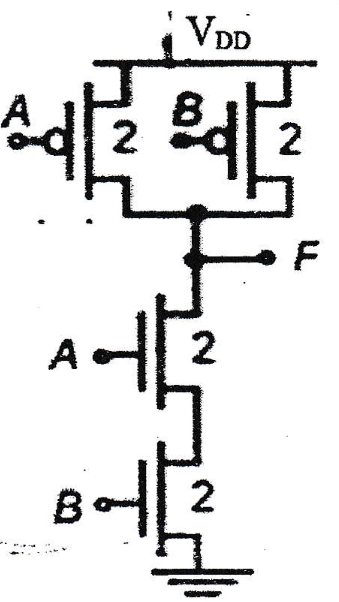
\includegraphics[height=4in]{images/es_1_76_Ba}
    \end{enumerate}

  \subsection{Programming Logic Device (PLD) IC Technology}
    \begin{enumerate}
      \item Describe the steps involved in design of Full-Custom, Semi-Custom and PLD. \hfill [8] (78 Po)

      \item Explain gate-array semi-custom IC technlogy and standard cell semi-custom IC technology. \hfill [4] (\bo{81 Ch})

      \item Draw the top-level diagram of a NAND gate using CMOS. \hfill [3] (\bo{80 Ch})

      \item What is photolithography? \hfill [1] (\texttt{81 Ash})
        \lb and what are its types? \hfill [4] (\texttt{80 Ash}, 72 Ma)

      \item Show various steps of photolithography process using appropriate diagrams. \hfill [5] (\texttt{82 Ka})

      \item Explain the importance of photolithography in IC manufacturing. \hfill [3] (79 Jth) [5] (\bo{74 Bh}, 73 Ma)
      \lb with suitable example. \hfill [8] (\bo{71 Bh})

      \item Describe the alignment and exposure techniques in photolithographic process in IC fabrication. \hfill [5] (71 Ma)

      \item Explain the basic steps of photo lithography process. \hfill [4] (\bo{78 Ch, 77 Ch}, 72 Ma) [5] (\bo{72 Ash}) [6] (\bo{76 Bh})
        \lb List the ten basic steps of photolithography. \hfill [3] (\texttt{81 Ash})
        \lb with appropriate figure. \hfill [4] (75 Ba)

      \item Explain Full-Custom, Semi-Custom and PLD schemes used in IC technology with steps and comparision. \hfill [8] (\bo{73 Bh})

      \item List the three major IC technologies with brief definitions. \hfill [3] (70 Ma)

      \item Draw final structurl view diagraam of respective structure. \hfill [5] (79 Jth)
        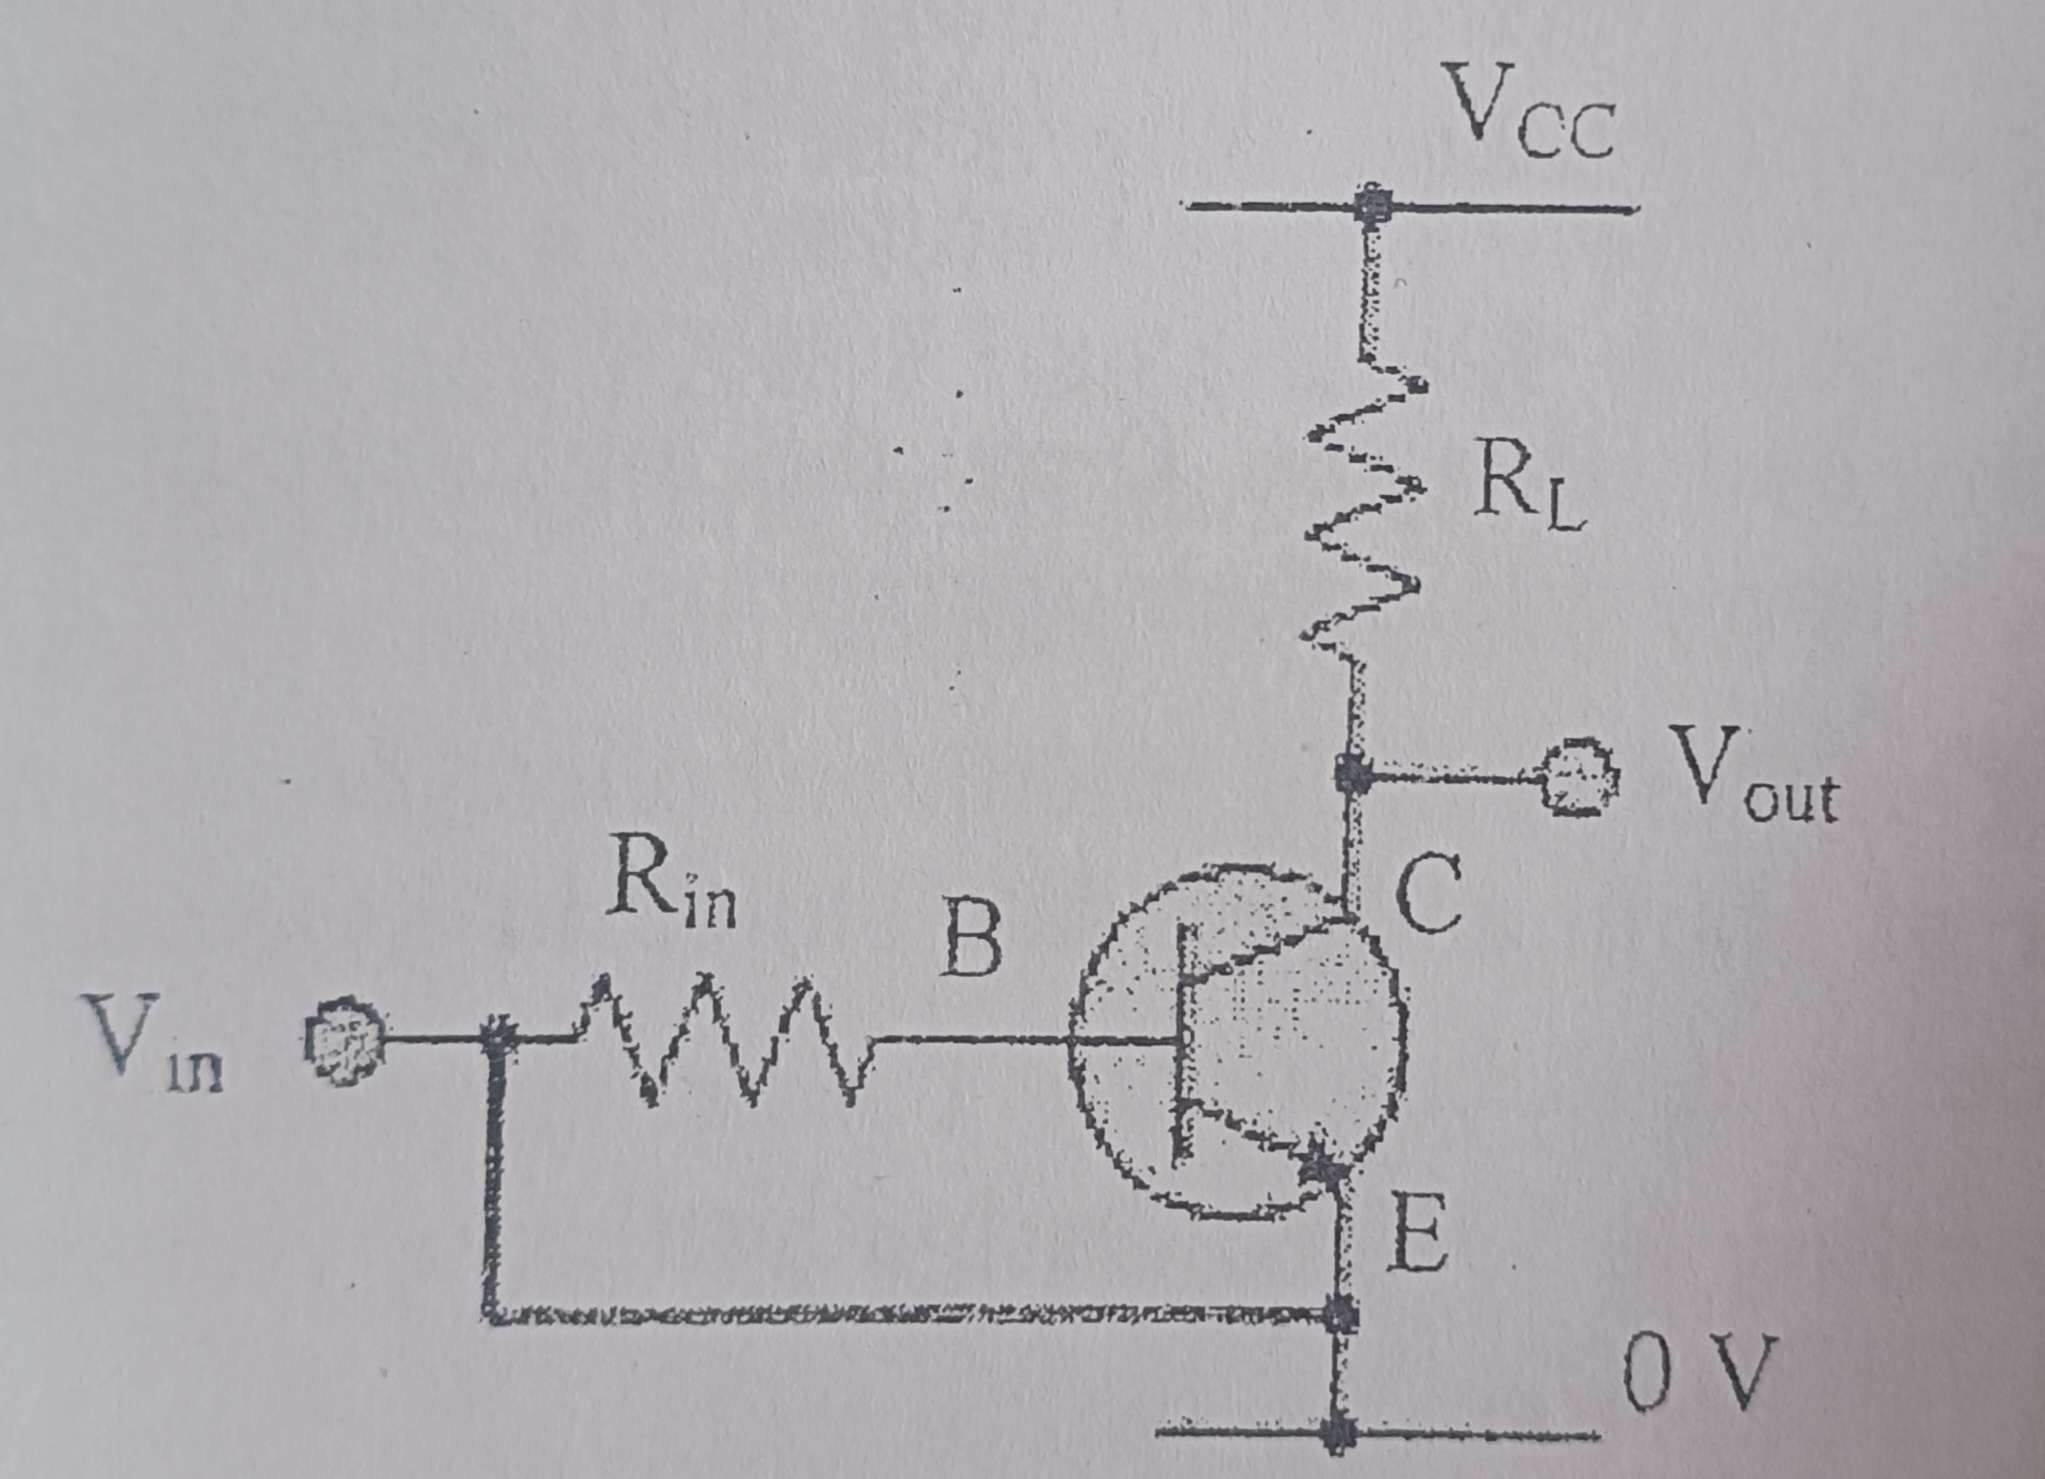
\includegraphics[width=4in]{./images/es_1_79_Jth.jpg}
    \end{enumerate}

\pagebreak

\section{Microcontrollers in Embedded Systems}
  \begin{center}(3 Hours / 8 Marks)\end{center}
  
  \subsection{Intel 8051 microcontroller family, its architecture and instruction sets}
    \begin{enumerate}
      \item How are microcontrollers different from microprocessors? \hfill [2] (\bo{78 Ch})

      \item What are the important operational features of 8051 microcontroller? \hfill [2] (\bo{80 Ch, 78 Ch}) [3] (\bo{73 Bh}) [4] (\bo{81 Ch})

      \item Draw the pin diagram of 8051 microcontroller and explain ports 1 and 2 only. \hfill [3] (\bo{72 Ash})

      \item Show the internal structure of the 8051 microcontroller. \hfill [4] (\bo{70 Bh})
        
      \item Explain the banks of register in 8051 microcontroller. \hfill [4] (\texttt{81 Ash})

      \item Explain data memory organization in 8051 microcontroller. \hfill [4] (\bo{79 Ch}, 78 Po)
      
      \item Which I/O (port based or bus based) is used in 8051 Microcontroller, describe. \hfill [2] (76 Ba)

      \item Explain port based and bus based I/O. \hfill [3] (72 Ma)

      \item Explain about PORT 3 of 8051 microcontroller. \hfill [2] (76 Ba)
        \lb about purpose of port 3 and port 2. \hfill [4] (79 Jth, 73 Ma)

      \item Explain the addressing modes used in 8051 microcontroller. \hfill [3] (\texttt{82 Ka})
        \lb with example. \hfill [4] (75 Ba, 72 Ma, 71 Ma)

      \item Provide a comparison chart of the 8051 family members. \hfill [4] (\bo{70 Bh})
    \end{enumerate}

  \subsection{Programming in Assembly Language}
    \begin{enumerate}
      \item Write a program to read an 8-bit temperature in Celsius from Port 1 and to output the Fahrenheit temperature equivalent onto port 2. (Note: F = C x (9/5) + 32) \hfill [5] (\texttt{82 Ka})

      \item Write an assembly language programming to alternatively blink the 8 LEDs connected at port 2 of the 8051 microcontroller. \hfill [4] (\bo{81 Ch}, 72 Ma)

      \item Write an assembly program for 8051 to count number of 0's in an 8-bit data stored in ROM at 40H and result in RAM at 41H. \hfill [4] (\bo{79 Ch})
        \lb rom at 75 H, ram at 45H. \hfill [4] (78 Po)

      \item Assume that XTAL = 11.0592 MHz, write a program to generate a square wave of 1 kHz frequency on pin P1.5 of 8051 microcontroller using timer. \hfill [2+4] (\bo{78 Ch})

      \item WAP to generate a square wave of 50\% duty cycle. \hfill [4] (\texttt{81 Ash})

      \item Generate a periodic square wave having a period of 15 ms and a duty cycle of 20\% in 8051 using assembly programming. The waveform should be produced at pin zero of port two (P2.0). The XTAL frequency is 11.0592 MHz and use Timer 1 in mode 0 (13-bit timer mode). \hfill [8] (\bo{76 Bh})

      \item Write an assembly program to design a down counter that counts from 99 to 00. \hfill [6] (\bo{77 Ch})

      \item Using 8051 instructions, control rate of blink of LED at pin P1.1 by two switches at P2.1 and P2.2 (One switch to increase rate of blink, another to decrease the rate of blink). \hfill [6] (76 Ba)

      \item Write an assembly language programming to blink 8 LED connected at Port 2 of 8051 microcontroller. \hfill [4] (75 Ba)

      \item Write an assembly language programming for 8051 microcontroller to read the data from switches connected at port 1 and send it to port 2 for display in LED. \hfill [4] (79 Jth, 73 Ma)

      \item Write a program in assembly language that computes a precise 5-millisecond delay using 8051 microcontroller. \hfill [4] (71 Ma)

      \item Write a program using C-programming language to find the sum between two 8-bit BCD data stored in RAM locations 50H and 51H and store the BCD sum at RAM locations 52H and 53H. \hfill [5] (\bo{72 Ash})
    \end{enumerate}
    
  \subsection{A simple interfacing example with 7 segment display}
    \begin{enumerate}
      \item What is seven segment display and write its types. \hfill [2] (\bo{75 Bh})

      \item Explain different configuration for seven segment display. \hfill [2] (\bo{77 Ch}, \texttt{80 Ash})

      \item Write an Assembly language program to display 9 to 0 in common anode 7-segment display connected at port 1 and show interfacing diagram also. \hfill [6] (\bo{80 Ch})
      \lb Write an assembly program to display 0 to 9 in seven segments display. \hfill [5] (\bo{73 Bh})

      \item Design a circuit with 7 segments display which is used as a counter watch which display second and minute. \hfill [6] (\bo{75 Bh})

      \item Write an assembly and C program to display 0 to 9 in seven segment display. \hfill [8] (\bo{71 Bh})

      \item Write the code for BCD counter to display 0 to 9999 in seven segment using VHDL. \hfill [8] (\bo{80 Bh})

      \item Design a circuit with 7seg display that is used as 2 digit hexadecimal counter using port 1 for LSB and port 0 for MSB. The gap between consecutive vaules should be 2 ms using timer 0 in mode 1. \hfill [6] (\texttt{80 Ash})

      \item Write 8051 program and draw circuit diagram to display number from 99 to 00 in seven segment display. The program should be written in both assembly and C. \hfill [8] (70 Ma)
    \end{enumerate}

\pagebreak

\section{VHDL}
  \begin{center}(4 Hours / 8 Marks)\end{center}
  
  \subsection{VHDL overview}
    \begin{enumerate}
      \item How does a FPGA differ from a microcontroller? \hfill [1] (70 Ma)

      \item What is structural style of architecture in VHDL? \hfill [3] (\bo{81 Ch})

      \item Explain different models of VHDL. \hfill [3] (\bo{75 Bh})

      \item Define behavioral model. \hfill [3] (\bo{80 Ch})
      \lb Define behavioral modeling. \hfill [2] (72 Ma)

      \item How is behavioral modeling different from dataflow modeling? \hfill [2] (\texttt{80 Ash})
        \lb explain behavioral and dataflow. \hfill [3] (78 Po)

      \item Explain different architecture model of VHDL. \hfill [2] (\bo{79 Ch})

      \item What's the use of VHDL code in embedded system? \hfill [2] (76 Ba)

      \item Explain COMPONENT with its declaration. \hfill [3] (75 Ba)

      \item Explain PROCESS in VHDL. \hfill [2] (\texttt{80 Ash}) [3] (73 Ma)

      \item Explain entity and architecture of VHDL declaration. \hfill [4] (79 Jth)

      \item How entity is declared in VHDL programming? \hfill [3] (71 Ma)

      \item Define data flow model. \hfill [2] (\texttt{81 Ash})
    \end{enumerate}

  \subsection{Finite state machine design with VHDL}
    \begin{enumerate}
      \item Write a VHDL code for a JK flip-flop. \hfill [5] (\bo{81 Ch})
      \lb using PROCESS. \hfill [5] (78 Po, 75 Ba)

    \item Write VHDL code for a D flip flop using process. \hfill [4] (79 Jth)

      \item Write a VHDL code for 4-bit BPA in structural model. \hfill [5] (\bo{80 Ch})

      \item Write a VHDL code to design a traffic light controller unit with necessary assumptions using state machine. \hfill [6] (\bo{79 Ch})

      \item Draw the state diagram for a sequence detector for the sequence 1011 and then develop a VHDL code based on the state diagram. \hfill [5] (\bo{78 Ch})

      \item Using structural model, write a code in VHDL to implement full adder. \hfill [8] (\bo{77 Ch})

      \item Write a VHDL code for a full adder using two half adders and one OR gate in structural model. \hfill [5] (\bo{75 Bh})
      \lb Write a VHDL code for a full adder using 2 half adder as component. \hfill [5] (73 Ma)

      \item Write an algorithm and VHDL code for custom single purpose processor that calculates the Greatest Common Divisor (GCD). \hfill [8] (\texttt{82 Ka})
        \lb of two numbers as Finite State Machine. \hfill [6] (\bo{76 Bh}) [2+6] (\bo{73 Bh}) [3+5] (\bo{71 Bh})

      \item Write VHDL code for a factorial processor showing its algorithm and state diagram. \hfill [2+6] (\texttt{81 Ash})

      \item Design and write a code for Decoder using VHDL. \hfill [6] (76 Ba)
      
      \item Write VHDL code for 2-input multiplexer. \hfill [6] (72 Ma)

      \item Write VHDL code to implement 1:8 Demux. \hfill [4] (\texttt{80 Ash})

      \item Write an algorithm and VHDL code for a custom processor that calculates LCM of two numbers. \hfill [5] (\bo{72 Ash})

      \item A circuit composed of two T-flip flops and an inverter shown in figure below, convert it to VHDL code. \hfill [5] (71 Ma)\\
      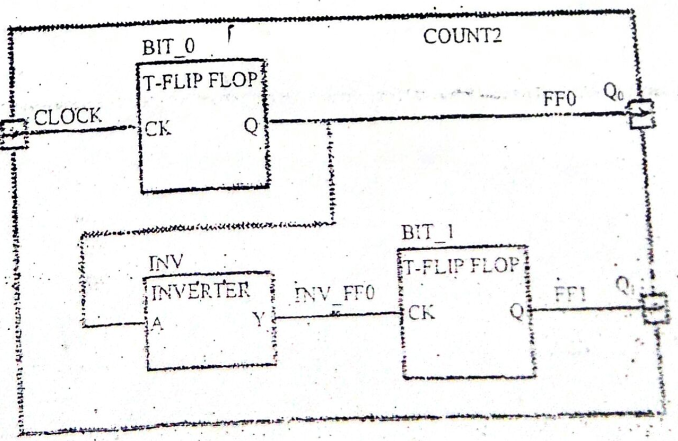
\includegraphics[width=4in]{images/es_2_71_Ma}

      \item Design a sequence detector for the string ``1101", that outputs a one when the input matches this string, show the fSM and its VHDL implementation. \hfill [7] (70 Ma)
    \end{enumerate}

\end{document}
